\section{问题三模型建立与求解}
\label{sec:question3}

\subsection{问题三分析}

问题三增加0、6、12、18时发布的未来24小时光伏预报，并允许修订未执行的常规购电计划。本问采用双时间尺度结构：外层按交易时点修订合同，内层每10分钟根据实际负荷、光伏与储电量执行充放电。

情景LP作为统一母模型，描述调整费用与历史误差；外层通过固定执行规则回放采购候选，在四个交易时点择优。求解结果分别检验筛选时点、信息来源与执行器的作用，并分析节费与紧急补购的权衡。

\subsection{问题三模型建立}

\begin{modelsummary}{问题三模型汇总}
\textbf{输入：}当期预报、历史残差、分时电价、实测SOC、零时计划与当前合同。\par
\textbf{决策：}四个交易时点选择剩余购电合同，储能每10分钟按固定规则执行。\par
\textbf{目标：}最小化候选回放账单与期末库存偏离的加权评分。\par
\textbf{约束与输出：}供需采用$\ge$，满足SOC与功率界；原计划全额计费、调整以零时计划为基准，输出有效合同、储能轨迹及实际账单。
\end{modelsummary}

\subsubsection{结算口径、实际账单与下调支配性}
\label{sec:settlement_mechanism}

记$g_{D,t}$、$a_{D,t}$和$h_{D,t}$分别为日期$D$的零时计划、最后生效常规购电量与紧急购电量，单位均为kWh，$[x]_+=\max\{x,0\}$。按题目给出的计划量计费、1.5倍上调、50\%下调违约费及5倍紧急费用，采用原计划全额付款且取消部分不退款的主口径；退款解释另作敏感性对照。

\begin{table}[htbp]
\centering\small
\caption{问题三两种结算口径及单时段示例（不含紧急购电费）}
\label{tab:mech_settlement_convention}
\begin{tabularx}{\linewidth}{p{0.18\linewidth}Xrr}
\toprule
口径 & 非紧急费用 & 下调示例 & 上调示例\\
\midrule
主口径：不退款 & $pg+1.5p[a-g]_++0.5p[g-a]_+$ & 110元 & 130元\\
退款敏感性口径 & $p\min\{g,a\}+1.5p[a-g]_++0.5p[g-a]_+$ & 90元 & 130元\\
\bottomrule
\end{tabularx}
\par\smallskip\parbox{\linewidth}{\footnotesize 两例均取$g=100$ kWh、$p=1$元/kWh；下调时$a=80$ kWh，上调时$a=120$ kWh。退款解释仅返还取消部分的原计划费用，紧急费用在两种口径下均另加$5ph$。}
\end{table}

主口径的当日真实账单为
\begin{equation}
 C_D=\sum_{t=0}^{143}p_{D,t}\left(g_{D,t}+1.5[a_{D,t}-g_{D,t}]_+
 +0.5[g_{D,t}-a_{D,t}]_++5h_{D,t}\right).
 \label{eq:settlement}
\end{equation}
调整费以零时原计划为基准，按最后生效量一次结算。实际账单分为计划、调整和紧急三项，终端罚项仅用于优化评分。

在正电价、原计划不退款、允许免费弃余时，下调受到支配。若$a_t<g_t$，令$a'_t=g_t$并弃置多出的$g_t-a_t$，保持充放电、紧急购电和SOC不变，仍满足物理约束，费用减少$0.5p_t(g_t-a_t)>0$。故至少存在满足$a_t\ge g_t$的最优解；退款口径的采购响应另行检验。

\subsubsection{由1.5倍增购费用推导条件采购阈值}

沿用问题二的无储能单时段分析，设$X$为修订时未知的实际净需求，$p>0$，并固定原计划$g\ge0$。在主口径下只需考虑$a\ge g$，已承诺的$pg$为常数，因此当前增购决策为
\begin{equation}
 J_3(a)=1.5p(a-g)+5p\,\mathbb E[(X-a)_+],\qquad a\ge g.
 \label{eq:mech_q3_cost}
\end{equation}
其中概率和期望均以该次修订已经获得的信息为条件。设$F_X(x)=\Pr(X\le x)$、$F_X(x^-)=\Pr(X<x)$，则
\begin{equation}
 \partial J_3(a)=p[5F_X(a^-)-3.5,\ 5F_X(a)-3.5].
 \label{eq:q3_adjustment_subgradient}
\end{equation}
内点$a>g$的最优条件为$F_X(a^-)\le0.7\le F_X(a)$，边界$a=g$的最优条件为$F_X(g)\ge0.7$。按下分位数定义，可取
\begin{equation}
 \begin{cases}
 a_3^\star=\max\{g,F_X^{-1}(0.7)\},\\[2pt]
 a_3^\star-g=[F_X^{-1}(0.7)-g]_+.
 \end{cases}
 \label{eq:mech_q3_quantile}
\end{equation}
上述次梯度条件同时覆盖离散与连续分布；连续内点满足$1.5p-5p\Pr(X>a)=0$。70\%刻画无储能、给定原计划后的最终有效购电量阈值，增购量为其超过$g$的部分。含储能调度通过联合优化处理跨时段库存价值。

\subsubsection{合法信息更新与外层滚动采购模型}

用十分钟物理索引表示外层时点，令$\mathcal T_u=\{0,36,72,108\}$。在$\tau\in\mathcal T_u$读取实测储电量$e_\tau^{\rm act}$，只处理$\tau,\ldots,143$的未执行区间；已执行动作及费用保持不变。光伏采用该时点刚发布的预报，负荷零时预测采用一月已选定的最近两个同星期日均值。为利用已经观察到的当天负荷偏差，在$\tau>0$时计算
\begin{align}
 b^L_{D,\tau}&=\frac{1}{12}\sum_{k=\tau-12}^{\tau-1}
       (L_{D,k}-\widehat L^{(0)}_{D,k}),\label{eq:q3_load_bias}\\
 \widehat L^{(\tau)}_{D,t}&=\max\left\{0,\widehat L^{(0)}_{D,t}+
 \operatorname{clip}\!\left(b^L_{D,\tau}e^{-(t-\tau+1)/36},
       -0.3\widehat L^{(0)}_{D,t},0.3\widehat L^{(0)}_{D,t}\right)\right\},\quad t\ge\tau.
 \label{eq:q3_load_update}
\end{align}
$\operatorname{clip}(x,l,u)=\min\{u,\max\{l,x\}\}$。该预定规则使用此前两小时实测偏差，按六小时尺度衰减，并限制在零时预测的$\pm30\%$。

在同一发布时间、相同剩余时域内提取此前最多28个完整日的净负荷残差，形成$n_{t,s}$及概率$\pi_s$。保留整日残差片段能表示连续偏高或偏低的误差。母模型在零时求解问题二式\eqref{eq:q2_objective}的经济场景模型；后续时点以已选定的零时计划$g_t$为基准，令$a_t-g_t=u_t^+-u_t^-$，$u_t^+,u_t^-\ge0$，求解
\begin{align}
 \min\quad &\sum_{t=\tau}^{143}\bar p_t(1.5u_t^++0.5u_t^-)
 +\sum_s\pi_s\sum_{t=\tau}^{143}5p_{t,s}h_{t,s}
 +\beta_T|e_{144}-6000|,\label{eq:q3_revision_objective}\\
 \text{s.t.}\quad&\begin{cases}
 a_t+d_t+h_{t,s}-c_t\ge n_{t,s},\\
 a_t,h_{t,s}\ge0,
 \end{cases}
                    \label{eq:q3_revision_balance}\\
 &\begin{cases}
 a_t-g_t=u_t^+-u_t^-,\\
 u_t^+,u_t^-\ge0,\\
 e_\tau=e_\tau^{\rm act},
 \end{cases}\label{eq:q3_revision_contract}
\end{align}
并满足式\eqref{eq:soc}、\eqref{eq:limits}的储能约束。问题三$p_{t,s}=\bar p_t=p_t$为已知分时电价，场景价格记法供问题四沿用。原计划费是当前修订中的常数，优化时略去、结算时全额计入。取$\beta_T=\operatorname{median}_{t\ge\tau}\bar p_t$，以$e_{144}-6000=z^+-z^-$、$z^+,z^-\ge0$线性化绝对值，用软罚项估计剩余库存价值。

外层参考充放电和SOC在场景间共享，$h_{t,s}$为场景补救量；预定设置为28场景、零附加风险和零参考备用。每次求解当天全部剩余合同，执行至下一合法更新时间，再修订未执行部分。共享储能的规划费用与实际执行费用通过下述回放衔接。

\subsubsection{基于执行规则回放的购电候选筛选}
\label{sec:q3_candidate_screening}

候选集合$\mathcal K_\tau$在零时包含原情景LP、合法点预测LP，以及净需求预测增加$0.25\sigma_t$、$0.5\sigma_t$、$1.0\sigma_t$的三个余量LP。其中$\sigma_t^2=\sum_s\pi_s(n_{t,s}-\sum_j\pi_jn_{t,j})^2$，$\sigma_t$以kWh计；余量方案保持点预测价格不变。日内另加入“保持当前剩余有效合同”，沿用此前修订后尚未执行的合同。各LP采用相同实测SOC、物理约束及零风险、零备用设置，产生的购电量统一交由回放评分。

记候选剩余购电量为$q_t^{(k)}$。各候选从$e_\tau^{\rm act}$出发，在同一组历史情景上按式\eqref{eq:execute_charge}、\eqref{eq:execute_discharge}回放，得到$h_{t,s}^{(k)}$与$e_{144,s}^{(k)}$，并满足$q_t^{(k)}+d_{t,s}^{(k)}+h_{t,s}^{(k)}-c_{t,s}^{(k)}\ge n_{t,s}$。附件功率乘$\Delta t=1/6$ h换算为kWh后，直接乘电价计费。剩余时域账单为
\begin{align}
 C_{\tau,s}^{\mathrm{replay},(k)}
 &=\sum_{t=\tau}^{143}p_{t,s}\bigl(B_{\tau,t}^{(k)}+5h_{t,s}^{(k)}\bigr),
 \label{eq:q3_replay_bill}\\
 B_{\tau,t}^{(k)}&=
 \begin{cases}
 q_t^{(k)},&\tau=0,\\[1ex]
 g_t+1.5[q_t^{(k)}-g_t]_++0.5[g_t-q_t^{(k)}]_+,&\tau>0.
 \end{cases}\notag
\end{align}
其中$B_{\tau,t}^{(k)}$为非紧急计费等效电量：零时按候选计划量全额付费，日内计入原计划费及相对零时计划的调整费。已执行区间作为共同常数略去。

统一评分选择为
\begin{align}
 k_\tau^*&=\arg\min_{k\in\mathcal K_\tau}\sum_s\pi_s
 \left[C_{\tau,s}^{\mathrm{replay},(k)}
 +\beta_\tau\left|e_{144,s}^{(k)}-6000\right|\right],
 \label{eq:q3_candidate_score}\\
 \beta_\tau&=\operatorname{median}_{t\ge\tau}\sum_s\pi_sp_{t,s}.\notag
\end{align}
各候选共用情景、权重、初态、执行器、结算规则和终端系数。末库存偏离先逐情景取绝对值再加权，仅计入评分。零时将$q^{(k_0^*)}$保存为$g$，日内更新剩余有效合同。评分相同时按固定顺序选择，优先保留情景LP。

回放将当前合同固定至午夜，采用当前情景评估剩余日费用；实际运行在下一合法时点读取新信息并重新决策。最终方案在$\mathcal T_u$的四个时点均启用筛选。

固定合同内层LP及跨日续接用于检验母模型的执行机制，模型与对照结果见\ref{app:controllers}。最终方案保持一月冻结的规则执行器，采购候选按同一执行规则的回放费用评分。

\subsection{问题三求解}

\subsubsection{配置确定、滚动实施及费用统计}

预定经济基准为28场景、零风险与零备用，预测器和执行器在1月15--31日按实际账单选定。表\ref{tab:v2_controller_validation}给出未筛选母模型在相同初态、已选预测配置下的验证结果：规则费用919340.82元，剩余日LP为929987.84元，LP加跨日为920497.18元，据此冻结规则执行器，各组期末库存随表列出。候选筛选的适用问题及启用时点依据2--12月开发性回测确定，此后保持最终配置固定。

\begin{table}[htbp]\centering\small
\caption{相同已选预测配置下的执行器一月验证}
\label{tab:v2_controller_validation}
\begin{tabularx}{\linewidth}{LLRRR}\toprule
问题 & 执行器 & 实际费用/元 & 紧急量/kWh & 末库存/kWh\\\midrule
问题2 & 规则执行 & 917318.59 & 19.93 & 7155.31\\
问题2 & 储能LP & 928995.30 & 474.33 & 6000.00\\
问题3 & 规则执行 & 919340.82 & 49.23 & 7143.30\\
问题3 & 储能LP & 929987.84 & 195.13 & 6000.00\\
问题3 & 储能LP+跨日 & 920497.18 & 195.13 & 7143.30\\
问题4-2 & 规则执行 & 1042234.20 & 19.93 & 7298.41\\
问题4-2 & 储能LP & 1052652.76 & 19.93 & 6000.00\\
问题4-3 & 规则执行 & 1043044.13 & 44.10 & 7308.72\\
问题4-3 & 储能LP & 1057597.78 & 220.05 & 6000.00\\
问题4-3 & 储能LP+跨日 & 1047012.91 & 220.05 & 7291.46\\
\bottomrule\end{tabularx}
\par\smallskip\parbox{\linewidth}{\footnotesize 同一问题内使用相同1月15日期初库存，之后独立因果运行。费用不含终端罚项；末库存并不强制相等。}
\end{table}

使用HiGHS求解稀疏LP。零时生成并筛选原计划，6、12、18时依据新信息筛选剩余合同，储能每10分钟按实值执行，日末按式\eqref{eq:settlement}结算并传递$e_{D+1,0}=e_{D,144}$。原版一月轨迹提供固定前缀，同一问题的各方案从共同2月初态出发，随后独立、连续运行。

最终方案2月初态为8814.60 kWh，12月末为6240.32 kWh。334天计划费13503057.82元、调整费248699.70元、紧急费119713.93元，总费用13871471.44元。紧急购电21029.90 kWh，涉及119天、424个十分钟段，补购后逐段满足负载。实际日账单CVaR95为65552.76元，最高日费用67941.61元。相较问题二整体策略，总费用低1.0086\%、紧急量低75.26\%；两问采用各自的光伏预测、初态和采购配置。

\subsubsection{筛选时点消融与最终策略选择}
\label{sec:q3_screening_ablation}

固定预测、历史情景、执行器、结算和全部合法修订时点，比较不筛选、仅零时、仅日内及零时与日内均筛选四种配置。关闭筛选时仍用自身实测SOC与零时计划重解母模型LP，因此“仅零时筛选”仍保留6、12、18时的预测更新和采购修订。各组从共同初态连续运行，以计划、调整和紧急三项账单之和评价。

\begin{table}[htbp]\centering\small
\caption{候选筛选启用时点对实际总费用的影响}
\label{tab:outer_timing_ablation}
\begin{tabularx}{\linewidth}{LRR}\toprule
候选筛选配置 & 问题3总费用/元 & 问题4滚动版总费用/元\\\midrule
不启用筛选：母模型基线 & 13,975,810.86 & 14,769,232.53\\
仅零时启用 & 13,911,957.70 & 14,712,596.45\\
仅日内启用 & 13,947,087.88 & 14,734,593.23\\
\textbf{零时＋日内均启用：最终方案} & \textbf{13,871,471.44} & \textbf{14,670,237.87}\\
\bottomrule\end{tabularx}
\par\smallskip\parbox{\linewidth}{\footnotesize 各组均保留0、6、12、18时的合法预报更新与采购修订，仅改变是否启用候选筛选；关闭筛选时仍调用原情景优化模型。各方案从同一问题的共同初态出发，之后独立、连续推进状态，不每日重置。评价范围为2025年2月1日至12月31日，共334天。}
\end{table}


在2025年2月1日至12月31日的334天回测中，全时点筛选在表\ref{tab:outer_timing_ablation}的四种配置中费用最低。第三问较未筛选母模型13975810.86元节省104339.41元（0.747\%），较仅零时和仅日内分别节省40486.25元、75616.44元。第四问滚动版全时点费用14670237.87元，较母模型节省98994.66元（0.670\%），较仅零时和仅日内分别节省42358.58元、64355.36元。差值均由未舍入账单计算，据此保留两问的全时点配置。

\begin{table}[htbp]\centering\small
\caption{滚动采购候选筛选的费用与紧急补购权衡}
\label{tab:outer_screening_tradeoff}
\begin{tabularx}{\linewidth}{LLRRRR}\toprule
问题 & 配置 & 计划费/万元 & 调整费/万元 & 紧急费/万元 & 紧急量/kWh\\\midrule
问题3 & 母模型 & 1367.46 & 23.07 & 7.06 & 12647.76\\
问题3 & 最终方案 & 1350.31 & 24.87 & 11.97 & 21029.90\\
问题4滚动版 & 母模型 & 1446.02 & 24.19 & 6.71 & 11950.68\\
问题4滚动版 & 最终方案 & 1426.52 & 28.31 & 12.19 & 21293.41\\
\bottomrule\end{tabularx}
\par\smallskip\parbox{\linewidth}{\footnotesize 计划费按零时计划量全额结算，调整费始终以零时原计划为基准；紧急购电单独计费。终端偏离项不计入实际账单。两问题均以计划费用下降补偿新增调整费与紧急费。}
\end{table}


同一问题四组方案期末库存一致，第三问为6240.32 kWh、第四问滚动版为6274.99 kWh。表\ref{tab:outer_screening_tradeoff}显示，节费伴随更多紧急补购：第三问紧急量由12647.76增至21029.90 kWh，第四问滚动版由11950.68增至21293.41 kWh。第三问计划费减少171508.13元，超过新增调整费18034.75元与紧急费49133.97元；第四问滚动版计划费减少195001.12元，超过新增调整费41200.07元与紧急费54806.39元。

同一模块用于问题二和第四问日前版时，分别增费22571.98元（0.161\%）和63356.15元（0.428\%），故最终采用“日前两组保留母模型、滚动两组全时点筛选”。逐决策检查确认了可用信息范围、统一评分与连续执行。

\subsubsection{状态、新光伏及负荷反馈的逐层贡献}

本节以未筛选母模型独立检验信息来源。在相同初态、场景和规则执行器下，从仅零时外层计划出发，依次加入SOC更新、新光伏预报和已观测负荷偏差修正。四组均关闭候选筛选与跨日续接，“SOC-only”组仅沿用零时预测，各组按自身状态与合同连续运行。该实验与表\ref{tab:outer_timing_ablation}的筛选时点消融分别衡量信息来源和筛选模块的作用。

\begin{table}[htbp]\centering\small
\caption{问题3母模型的状态、光伏和负荷反馈分解}
\label{tab:v2_feedback}
\begin{tabularx}{\linewidth}{LRRRR}\toprule
策略 & 总费/万元 & 紧急量/kWh & 日费CVaR95/元 & 末库存/kWh\\\midrule
仅零时外层计划 & 1416.90 & 80181.62 & 71801.23 & 6240.32\\
仅更新SOC并重优化 & 1399.17 & 39298.96 & 66748.14 & 6240.32\\
再加入新光伏预报 & 1407.57 & 40071.16 & 66732.97 & 6240.32\\
再加入负荷偏差反馈 & 1397.58 & 12647.76 & 65518.79 & 6240.32\\
\bottomrule\end{tabularx}
\par\smallskip\parbox{\linewidth}{\footnotesize 未启用候选筛选的母模型对照；各组沿用原实验配置，覆盖334天并连续推进状态。}
\end{table}


仅零时外层计划费用14169011.89元，更新SOC后降至13991697.93元，减少177313.97元；加入新光伏后增至14075665.67元，增加83967.74元；再加入负荷偏差反馈后降至母模型13975810.86元，减少99854.81元。图\ref{fig:q3-feedback-waterfall}展示各阶段账单，反映新信息与采购、储能状态及预测误差的共同作用。

\begin{figure}[htbp]\centering
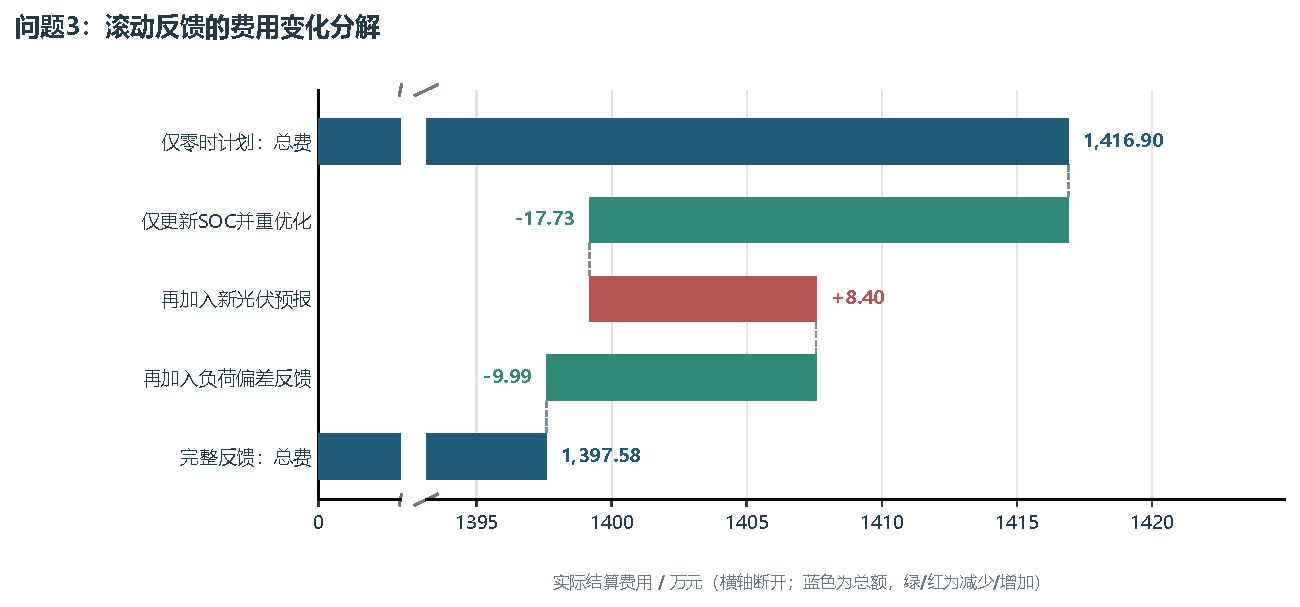
\includegraphics[width=0.94\linewidth]{figures/results/q3_feedback_waterfall.pdf}
\caption{未筛选母模型的逐层反馈费用分解（万元）。起止条从零累计至334天账单，中间条为相邻策略的闭环费用差；断轴放大账单附近的变化。}
\label{fig:q3-feedback-waterfall}
\end{figure}

\subsubsection{指定日期结果与实际运行轨迹}

图\ref{fig:v2-control}展示最终方案紧急量最大日7月4日的上调量、实际SOC与紧急量，并对照母模型的实际SOC。四个指定日的合同修订曲线见\ref{app:final_adjustments}，采购、储能与紧急量在下表完整列示。

\begin{figure}[htbp]\centering
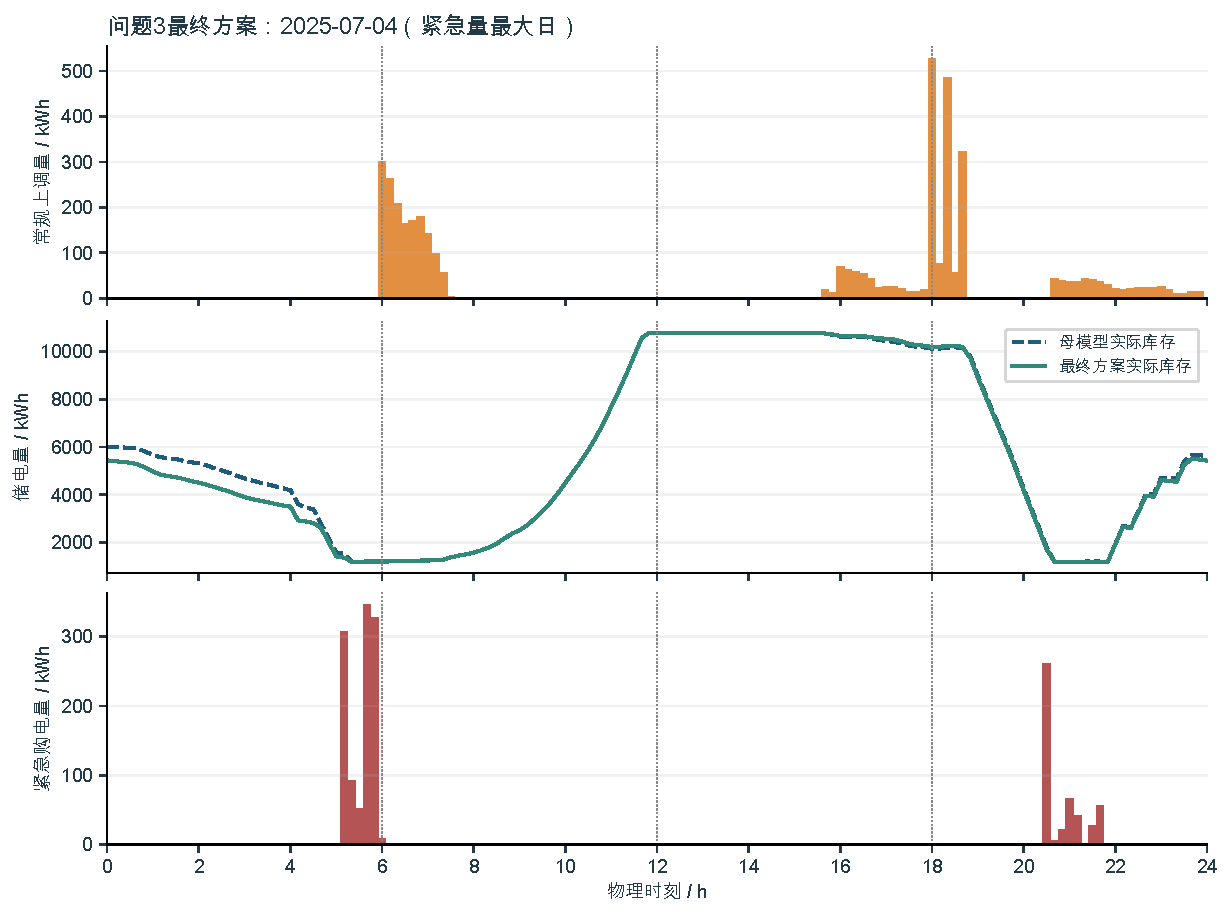
\includegraphics[width=0.95\linewidth]{figures/results/v2_control_difference.pdf}
\caption{问题三7月4日的最终购电调整、实际SOC与紧急量。库存图对照未筛选母模型，竖虚线标示6、12、18时修订时点。}
\label{fig:v2-control}
\end{figure}


\begin{table}[H]\centering\small
\caption{问题三指定日期购电结果（电量：kWh）}
\label{tab:q3-purchase}
\setlength{\tabcolsep}{4pt}
\begin{tabularx}{\linewidth}{lRRRR}\toprule
物理时段 & 03-20 & 06-21 & 09-23 & 12-21\\\midrule
10:00--10:10 & 0.00 & 0.00 & 0.00 & 0.00\\
12:00--12:10 & 624.29 & 0.00 & 444.81 & 1054.19\\
14:00--14:10 & 0.00 & 0.00 & 0.00 & 0.00\\
16:00--16:10 & 671.04 & 260.52 & 611.01 & 877.48\\
18:00--18:10 & 704.20 & 0.00 & 801.37 & 744.23\\
20:00--20:10 & 0.00 & 0.00 & 0.00 & 0.00\\
\midrule
全天常规量 & 71789.01 & 37273.13 & 73472.67 & 101747.42\\
全天实际费用/元 & 45563.84 & 21986.55 & 46201.57 & 65702.81\\
\bottomrule\end{tabularx}
\par\smallskip\parbox{\linewidth}{\footnotesize 日期均为2025年；购电量为最终生效常规量，紧急量单列。实际费用包含计划、调整及紧急三项账单。}
\end{table}

\begin{table}[H]\centering\fontsize{10}{12}\selectfont
\caption{问题三指定日期储能结果（kWh）}
\label{tab:q3-battery}
\setlength{\tabcolsep}{4pt}
\begin{tabularx}{\linewidth}{lRRRR}\toprule
物理时段 & 03-20 & 06-21 & 09-23 & 12-21\\\midrule
00:00--04:00 & 4146.19 / 181.53 & 915.21 / 972.82 & 4692.99 / 53.14 & 4496.41 / 40.16\\
04:00--08:00 & 883.67 / 6201.85 & 511.20 / 4390.39 & 892.10 / 5612.58 & 762.28 / 1406.28\\
08:00--12:00 & 5765.88 / 2465.92 & 8439.30 / 0.00 & 6293.08 / 1896.62 & 6441.76 / 6526.43\\
12:00--16:00 & 5215.25 / 254.72 & 0.00 / 0.00 & 3282.98 / 403.62 & 5333.82 / 2222.97\\
16:00--20:00 & 1.31 / 5594.70 & 241.25 / 5157.72 & 15.07 / 5619.05 & 0.00 / 5526.27\\
20:00--24:00 & 5703.85 / 2960.43 & 6354.48 / 2485.90 & 5609.40 / 3045.21 & 5771.81 / 2842.53\\
\midrule
期初 / 期末库存 & 6505.69 / 6428.95 & 7879.99 / 8243.25 & 6006.02 / 6235.06 & 6797.85 / 6695.97\\
\bottomrule\end{tabularx}
\par\smallskip\parbox{\linewidth}{\footnotesize 六个时段行按“充电量 / 放电量”列示；末行为当日0时 / 24时库存。}
\end{table}

\begin{table}[H]\centering\small
\caption{问题三指定日期紧急购电}
\label{tab:q3-emergency}
\setlength{\tabcolsep}{4pt}
\begin{tabularx}{\linewidth}{lLR}\toprule
日期 & 物理区间 & 紧急电量/kWh\\\midrule
03-20 & 09:10--10:00 & 311.46\\
06-21 & 无 & 0.00\\
09-23 & 20:20--20:30 & 6.38\\
 & 20:50--21:10 & 67.74\\
 & 21:20--21:50 & 34.20\\
12-21 & 无 & 0.00\\
\midrule
四日合计 &  & 419.77\\
\bottomrule\end{tabularx}
\par\smallskip\parbox{\linewidth}{\footnotesize 各日合计依次为311.46、0.00、108.31、0.00 kWh。}
\end{table}

\begin{table}[H]\centering\small
\caption{问题3指定日期计划、调整与费用分解}
\begin{tabularx}{\linewidth}{lRRRRR}\toprule
日期 & 计划量/kWh & 生效量/kWh & 计划费/元 & 调整费/元 & 紧急费/元\\\midrule
2025-03-20 & 71671.98 & 71789.01 & 43906.14 & 136.18 & 1521.51\\
2025-06-21 & 37259.86 & 37273.13 & 21962.65 & 23.90 & 0.00\\
2025-09-23 & 73472.67 & 73472.67 & 45684.65 & 0.00 & 516.92\\
2025-12-21 & 101747.42 & 101747.42 & 65702.81 & 0.00 & 0.00\\
\bottomrule\end{tabularx}\end{table}


指定日期表、轨迹与全年工作簿由最终执行数组统一生成。四小时充放电量累加24个十分钟段，同一区间可包含不同时间的充、放电动作。计划页保存原计划费，调整页保存最后有效常规量及完整实际账单。
\FloatBarrier
